%!TEX program = xelatex
\documentclass[a4paper, zihao=-4,utf8]{ctexart}

\usepackage{graphicx, geometry}
\geometry{a4paper,left=2cm,right=2cm,top=1cm,bottom=1cm}
\graphicspath{{pic/}}

\title{给糙汉的一封信}

\begin{document}
\maketitle
提笔再三,终于鼓足精神写了这封信。和糙汉相处的点点滴滴,历历在目,仿佛昨日初见,又仿佛隔数十年(恍惚度日ing)。

不知道糙汉最近身子骨可好?是否一紧张加上工作忙就会胃疼,一日三餐都得按时吃哦。我爸是个沉默寡言的人,在我每次出远门时都只会叮嘱一句:要好好吃早饭!上次见面时见糙汉鼻头有些红,也记不清有没有问了。坐地铁上会用手按摩眼睛,怕也是长期对着电脑用眼过度,要记得多吃蔬果,像之前的黑莓、蓝莓等都是不错的花青素补充体。

老父亲模式 end。我时常觉得自己如上次发的 cheems 一样,跟这个世界有种莫名的疏离感。有时候要么无动于衷、冷眼旁观,要么紧张兮兮、过于严肃。我时常感觉到这个世界的不真实,比如荒诞可笑的防疫政策,比如现实和网络世界的参差,但我知道的是“现在捧着手机屏幕的糙汉,并不是幻影呀”。

第一眼见到糙汉的时候,就被那 2.8 米内无敌的气场给镇住了,我 … 一败涂地。等摘下了口罩,天哪,比照片还要漂亮、有仙女气,不禁先怵了三分在心头。但一张口,我放心了,这就是我喜欢的姑娘啊,从骨子里透出一股 …… 不服输的娇憨。甚至第一次见面我就想牵手呢!只是暂时忍住了,心底里觉得我们的缘分来日方长。很久没见过如此清新脱俗的女孩子,在走回西直门的路上,我就想把自己经历过的两段最闲适的旅行经历分享给你,一次是重庆,一次是天津。

非常真诚地说,在见了糙汉第一面之后,我就盼望能和糙汉相处在一起,每天的早晚安都是一天工作的动力源泉。慢慢地,我们从生活趣事聊到工作问题,从饮食聊到影视,小到做家务(也不小)和甜咸豆腐脑,大到生死抉择和育儿观。在高度统一了思想认知的前提下,发现了我俩兴趣爱好上的文艺与逗比,这何尝不是一种幸事呢。我们都对医学有一定的了解,哦,对了,糙汉的那句“粪便移植”直到现在依然在我脑中回响。有人说相亲就是给人打标签,可我默默放下了举着的标签,从兜里摸出了一张又藏了好几年的破布,摊开,定睛一看,上面两个大字——“老婆”。

吃哈根达斯和猪肋排的两次见面,糙汉换了不同风格的衣服,感受到了风情万种和勤俭节约。要说两人内心的交流,还得是在吃菌子的时候。看得出糙汉对于恋爱或是感情的不确定性有惶恐,在成熟的年岁可以轻松处理的问题,在稚嫩的时期仍然是不可承受之重。不仅仅是感情,还有校园欺凌和体罚等,忽然就理解了糙汉想要从事医学的心情。从这天起,糙汉开始频繁分享与舍友的精彩互动,有些理解糙汉的逗比和愤青,是跟这个世界抗争的一种形式。

也许糙汉理解的“文艺”是我和世界达成和解的一种方式,更深层的是我本人不善于表达,真的表达出来又往往是讲大道理(我都烦我自己)。借电影的口,讲我想说给这个世界听的话,用打分来投出自己的选票。如我前面所说的,我和这个世界有疏离感,躲到电影世界里才能感受到被包容和认可。

在天最热的时候回家了一波,这时糙汉却感冒了,记得那天凌晨无助的糙汉买药的情形,大概唤醒了我内心最深的恐惧。有个同学讲过,他加班到凌晨回家,突然心绞痛倒在客厅,缓了十分钟才爬起来,当时真是无助恐慌到了极点。我就会想,我在异乡怎么办?谁会帮我,我又能做什么来预防这些情况发生。我真的需要一个可以互相陪伴的人,我也真的需要认真锻炼身体,努力保持健康。

回来后突然得知糙汉可能要去上海出差,我 …… 暗暗压抑住了心中的不甘,老天爷呀,非要这样设置感情关卡吗?那时确实也暗暗做好了准备,因为渣男女友在上海,我们可以经常一起去上海。只是疫情往复,想必前路必不是坦途。所幸在每日插科打诨的日常下,有惊无险地度过了惴惴不安的一周。

8.20,我们牵手了。糙汉的手手好软,根本不像是会砰砰打拳的,幻想着拳头砸在身上一点都不疼(找死)。那天风好温柔,记得在前门等公交车的间隙,我看着糙汉的零星白发,心里不是滋味,但又表达不出。射箭前讲到了工作相关的问题,让我又有了些危机感,等出来了上了出租车,我们聊到了对今后相处的看法,得到了糙汉高度的评价,那时就暗下决心,不能辜负眼前这个女人。

走在回家的路上,牵着手,看着人来人往。走一次,走两次,走很多次……

之后就感觉糙汉在工作上忙起来了,经常说怎么比程序员还要累,真的很想替糙汉分担。但某天忽然感觉到糙汉对感情的疑虑,

\begin{figure}[htp]
  \centering
  \fbox{
    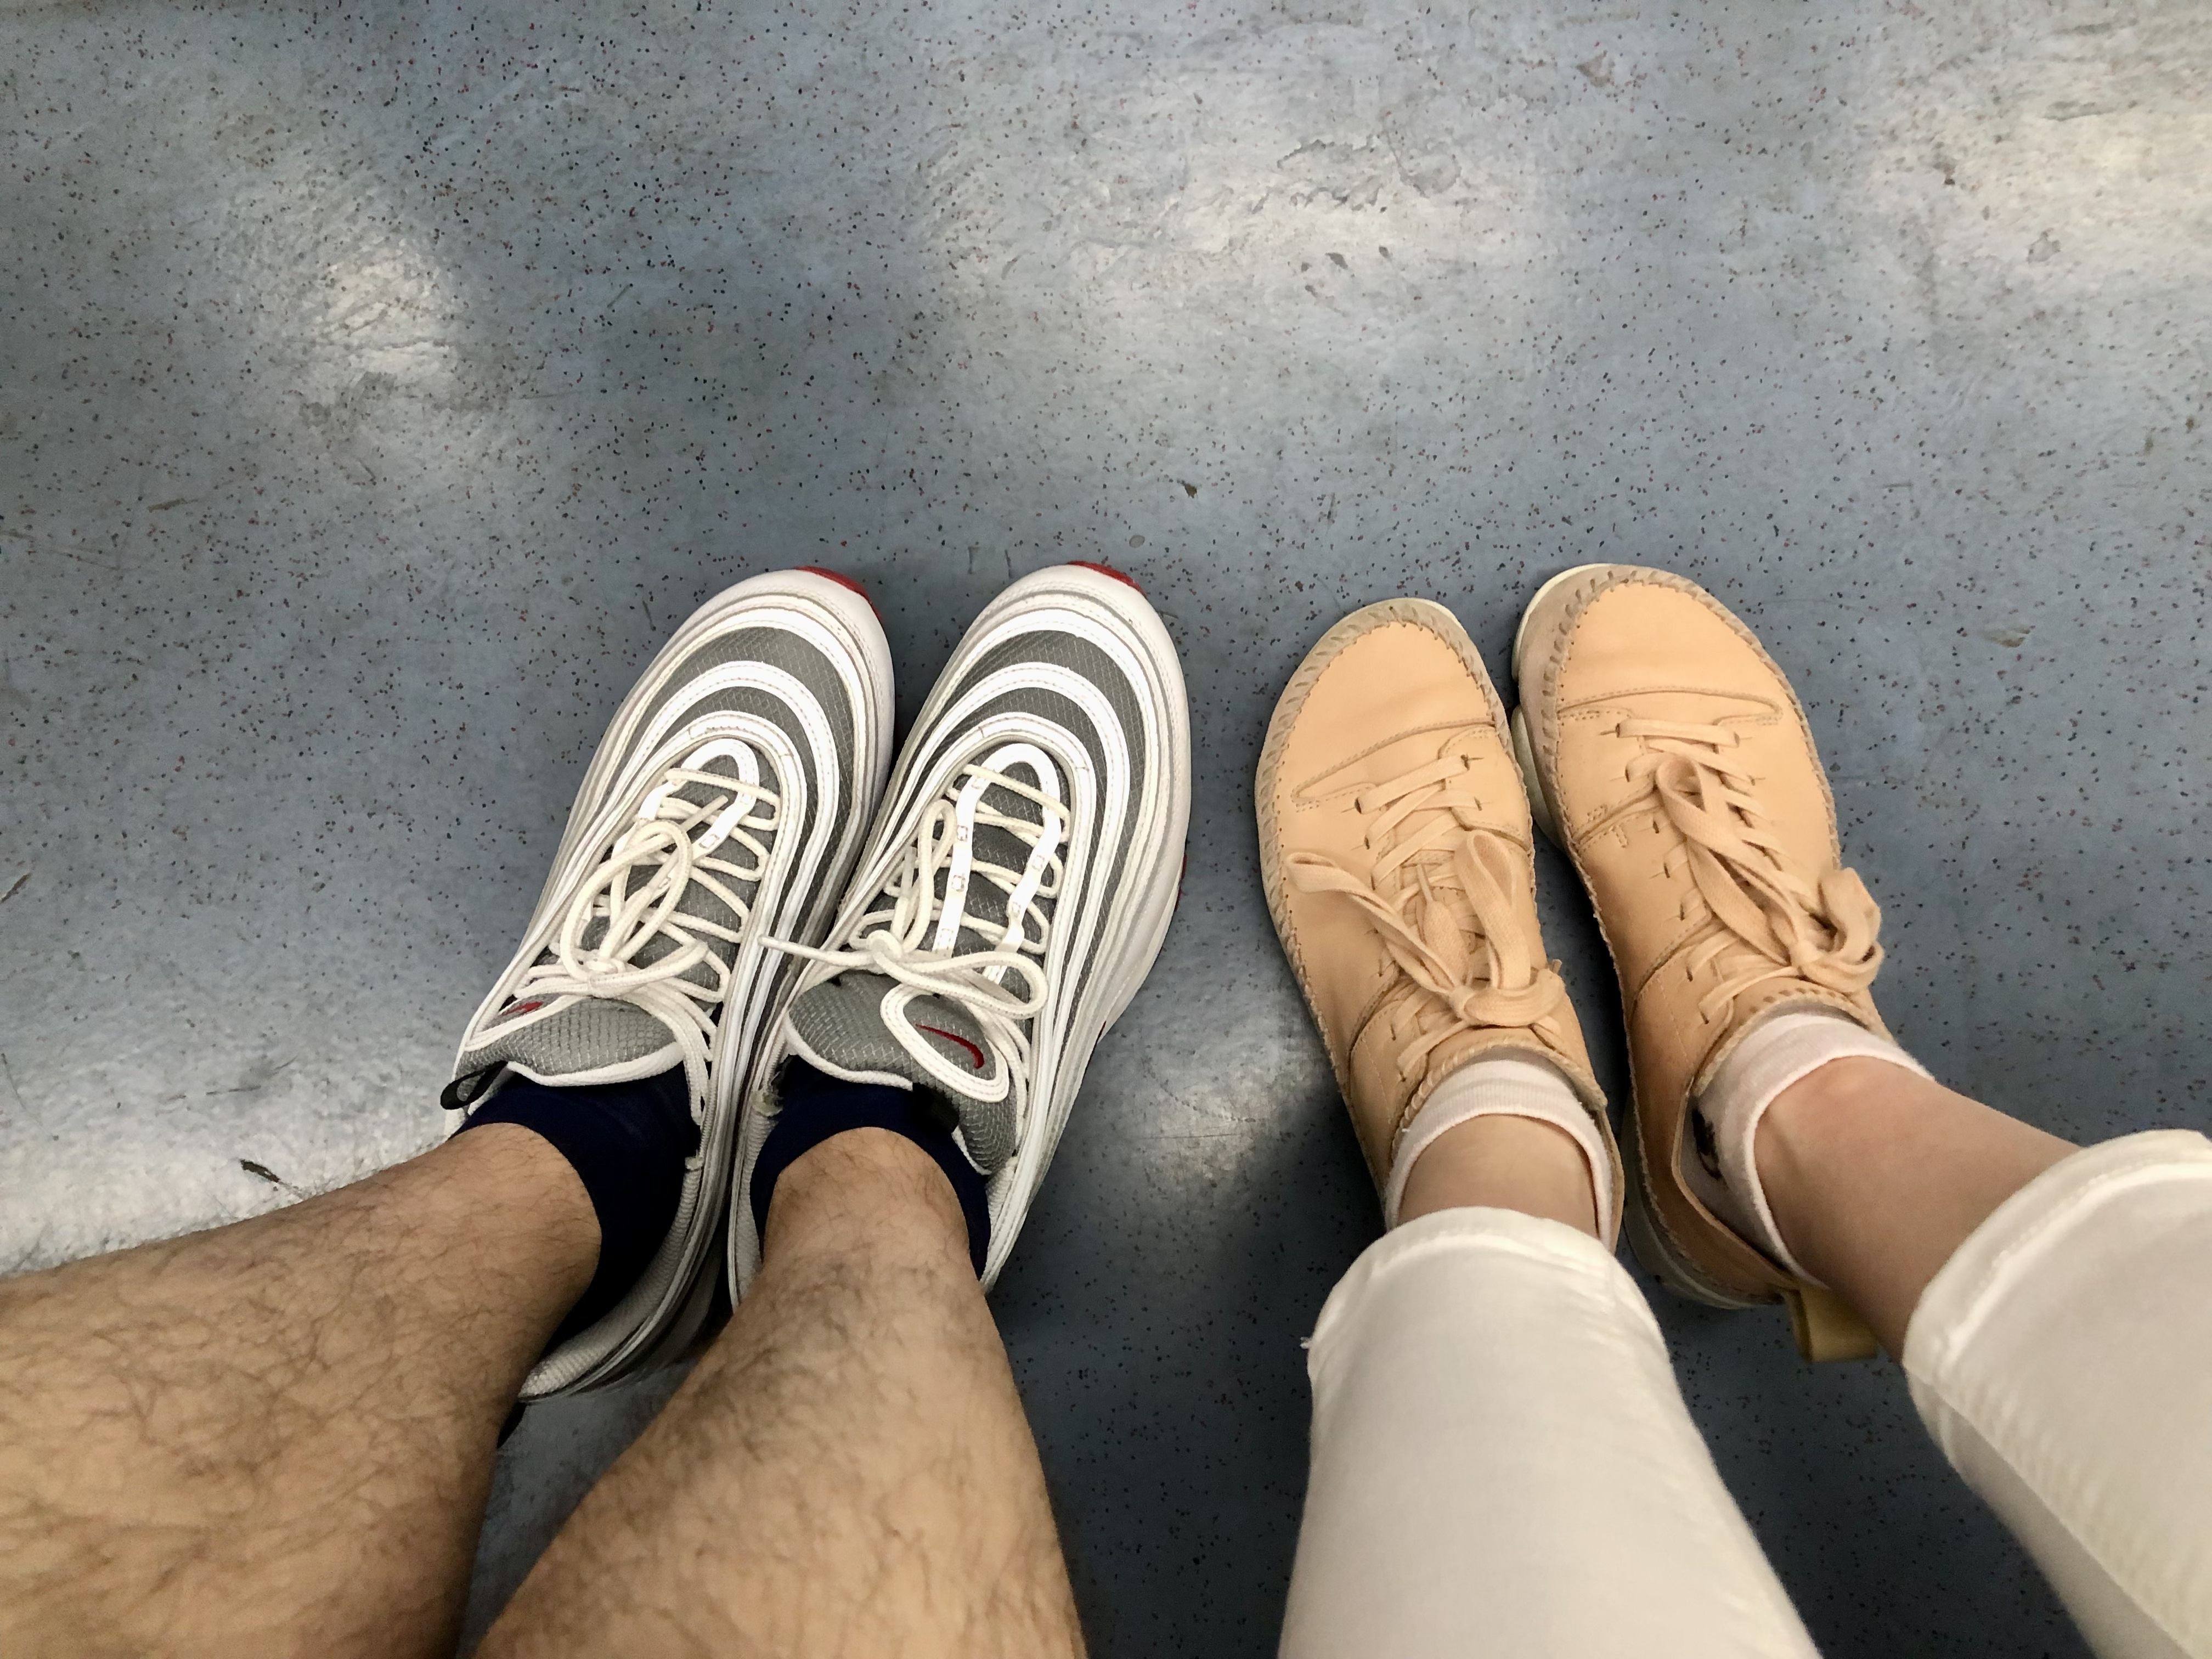
\includegraphics[width=.8\textwidth]{love.jpg}
  }
\end{figure}
\end{document}
